\section{Experiments}

\begin{itemize}[leftmargin=*]
    \item \textbf{RQ1:} Can self-proposed rubrics provide reliable rewarding signals for RL training?
    \item \textbf{RQ2:} How does RLCER enhance the reasoning capabilities of LRMs?
    \item \textbf{RQ3:} How does the self-evolving enable the rubricator to gradually propose better rubrics?
    \item \textbf{RQ4:} How effective are generated rubrics at facilitating LLM reasoning when used as in-prompt hints?
\end{itemize}

\subsection{Experiment Setup}
We briefly introduce the experiment setup of our paper, and more details can be found in Appendix \ref{apdx:impl-details}. 


\textbf{LLMs.} 
We conduct experiments on two open-source Qwen models of different sizes (8B and 4B) \cite{Qwen3}.
We first cold-start the pre-trained models (\ie Qwen3-8B-Base and Qwen3-4B-Base) by performing supervised fine-tuning on correctly formatted data obtained via reject sampling from a stronger teacher model, as we observe that even post-trained versions of such small-sized models (\eg Qwen3-8B) cannot always strictly follow the required instructions when acting as the rubricator and reasoner. 
More details can be found in Appendix \ref{apdx:impl-details}.
All subsequent RL experiments are conducted based on these carefully cold-started models.

\textbf{Training and evaluation.} 
We train models based on the DAPO-Math-17k dataset \cite{DAPO}, which contains 17k high-quality math questions. 
We evaluate models on various reasoning benchmarks.
For math reasoning, we evaluate math-reasoning benchmarks including AIME24 \cite{AIME}, AIME25 \cite{AIME}, and AMC23 \cite{aimo_amc_2023}.
For general knowledge reasoning, we evaluate on GPQA-Diamond \cite{GPQA} and SuperGPQA \cite{SuperGPQA}. 
For the large size of SuperGPQA, we evaluate on three subsets, each including 100 questions, namely SuperGPQA-Eng, SuperGPQA-Med, and SuperGPQA-Sci. 
For each testing question, we sample $N$=16 responses with sampling temperature as 0.7.
We report pass@1 as the accuracy metric (\ie the average pass rate among 16 responses).
For all RL training, we fix the max training steps to 1500.

% \clearpage
\subsection{(RQ1) Reliability of Self-Proposed Rubrics} \label{sec:rubrics-reliability}

\begin{wrapfigure}{r}{0.52\textwidth}
  \vspace{-10pt}
  \centering
  \begin{subfigure}[ht]{0.49\linewidth}
    \centering
    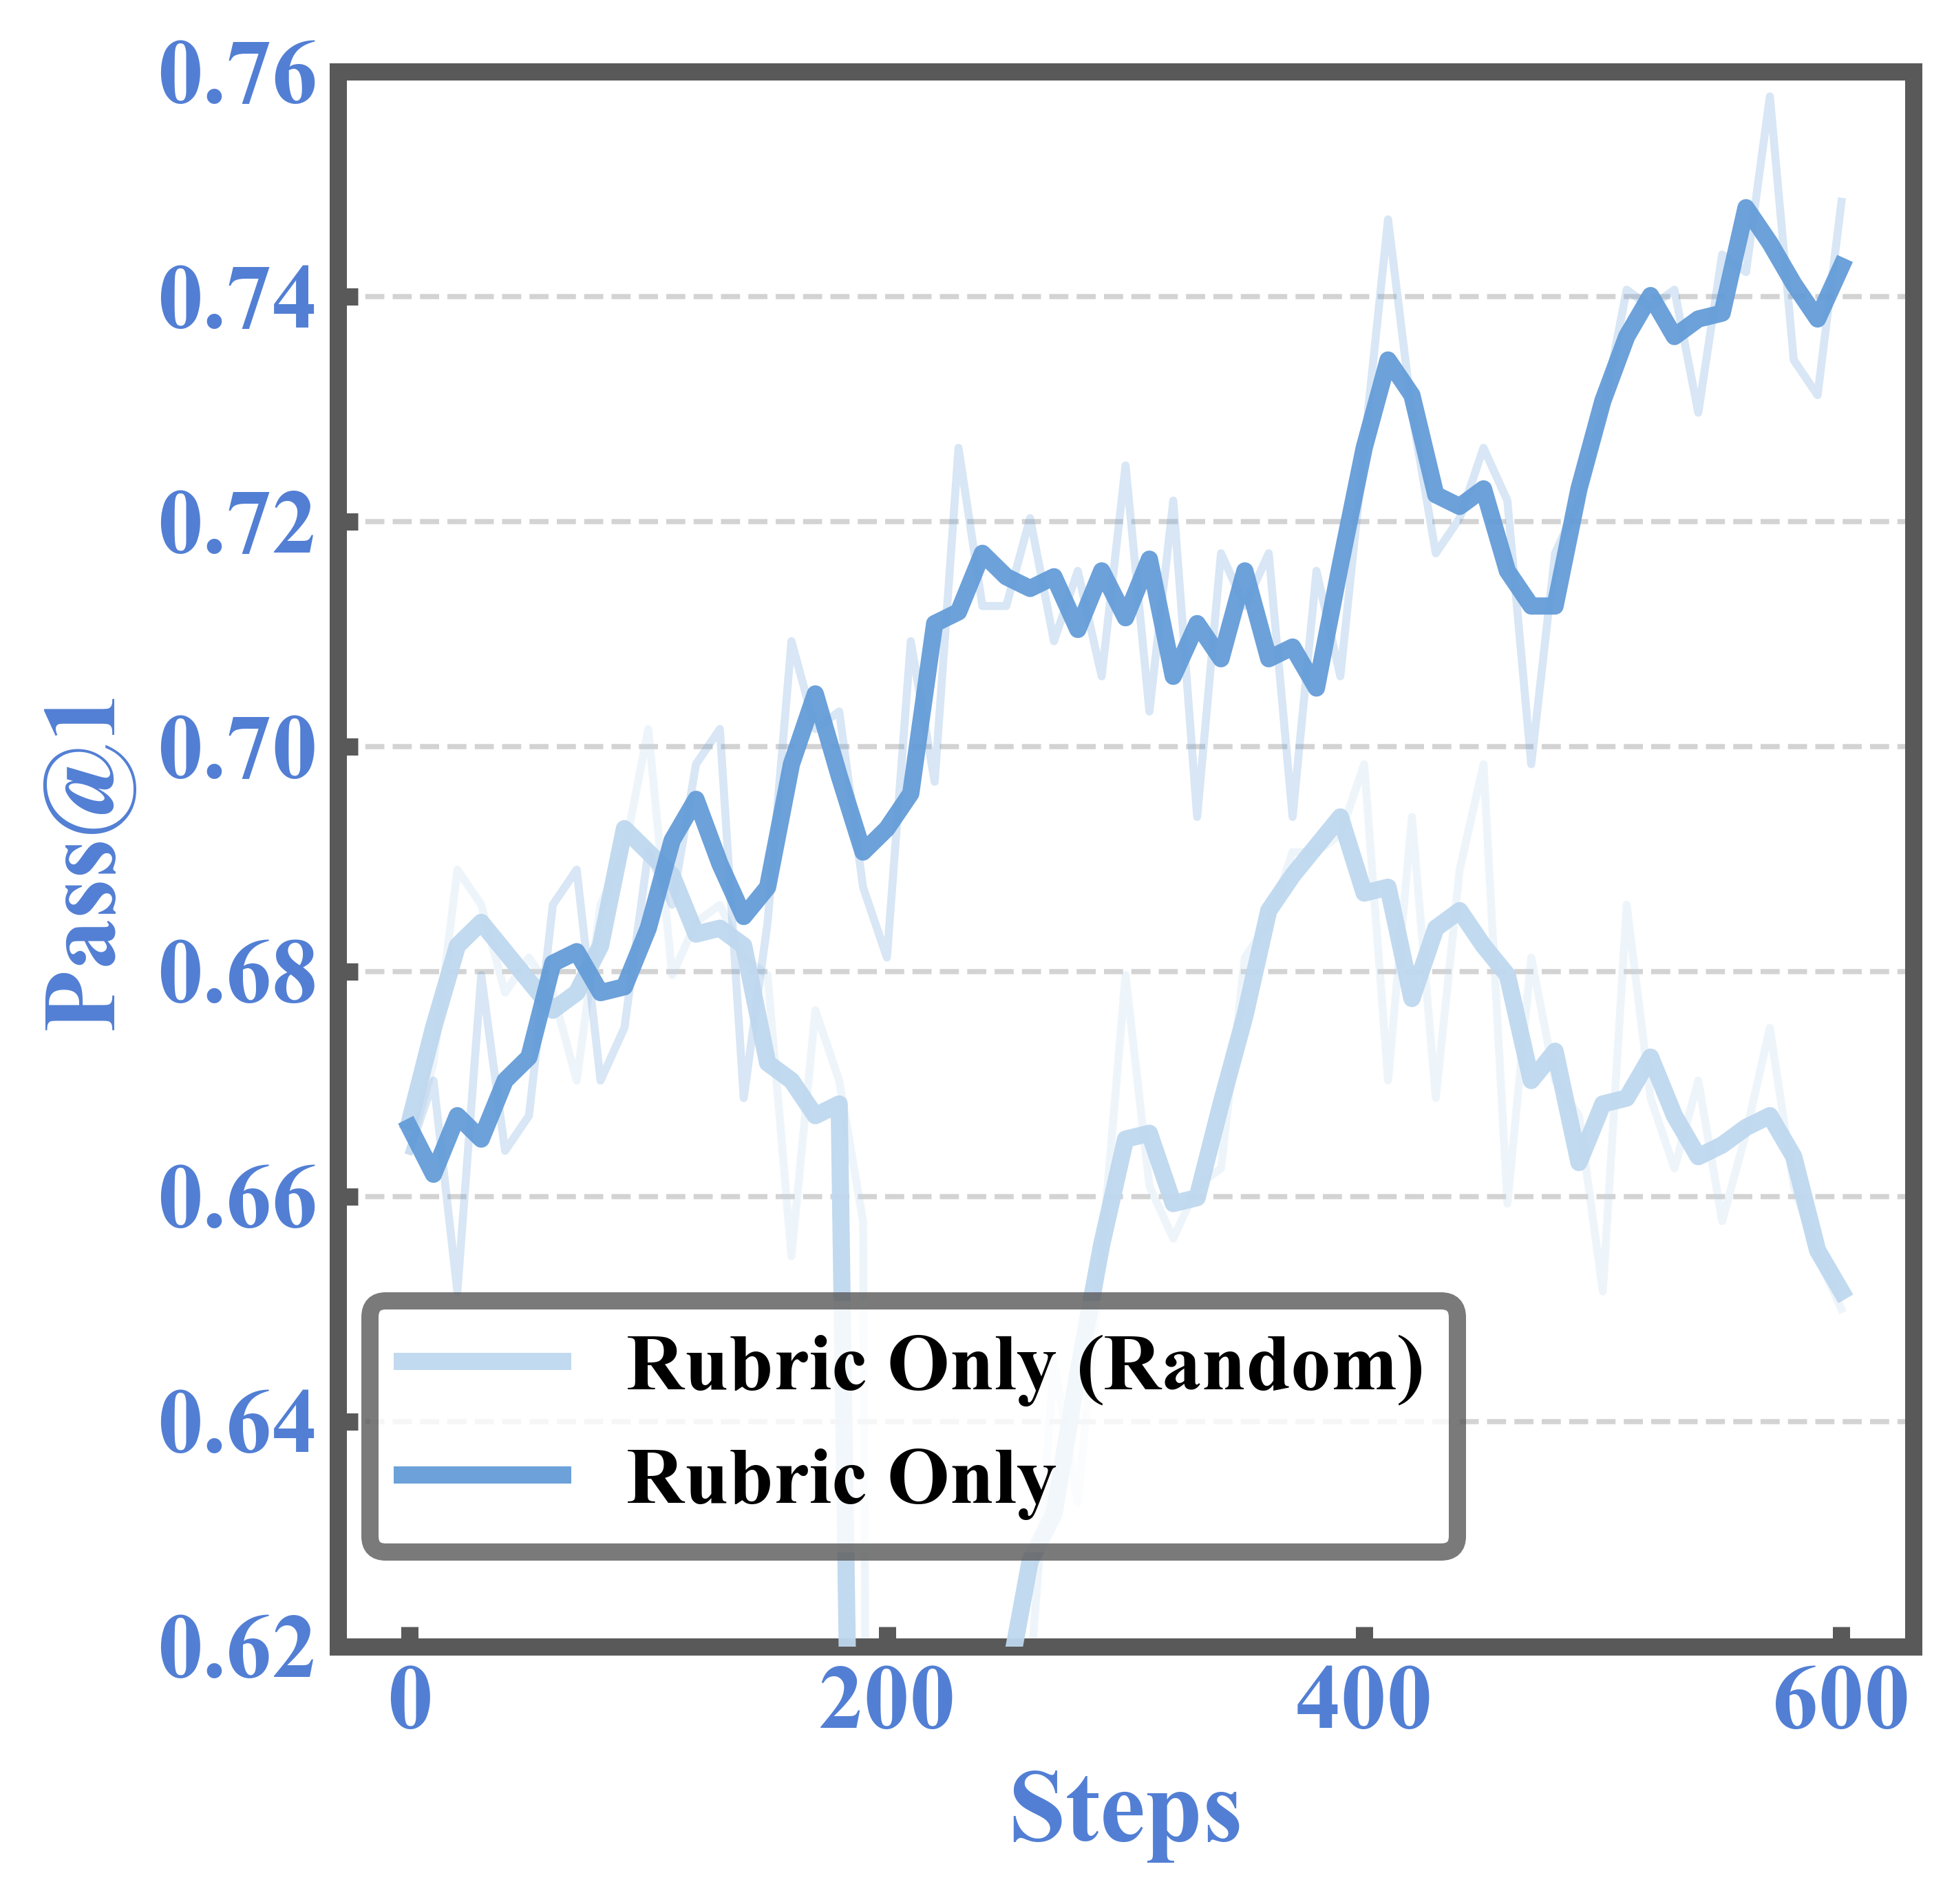
\includegraphics[width=\linewidth]{figures/exp/rubric_only/amc23_rubric_only.png}
    \caption{Accuracy on AMC23.}
    \label{fig:rubric-only-a}
  \end{subfigure}\hfill
  \begin{subfigure}[ht]{0.49\linewidth}
    \centering
    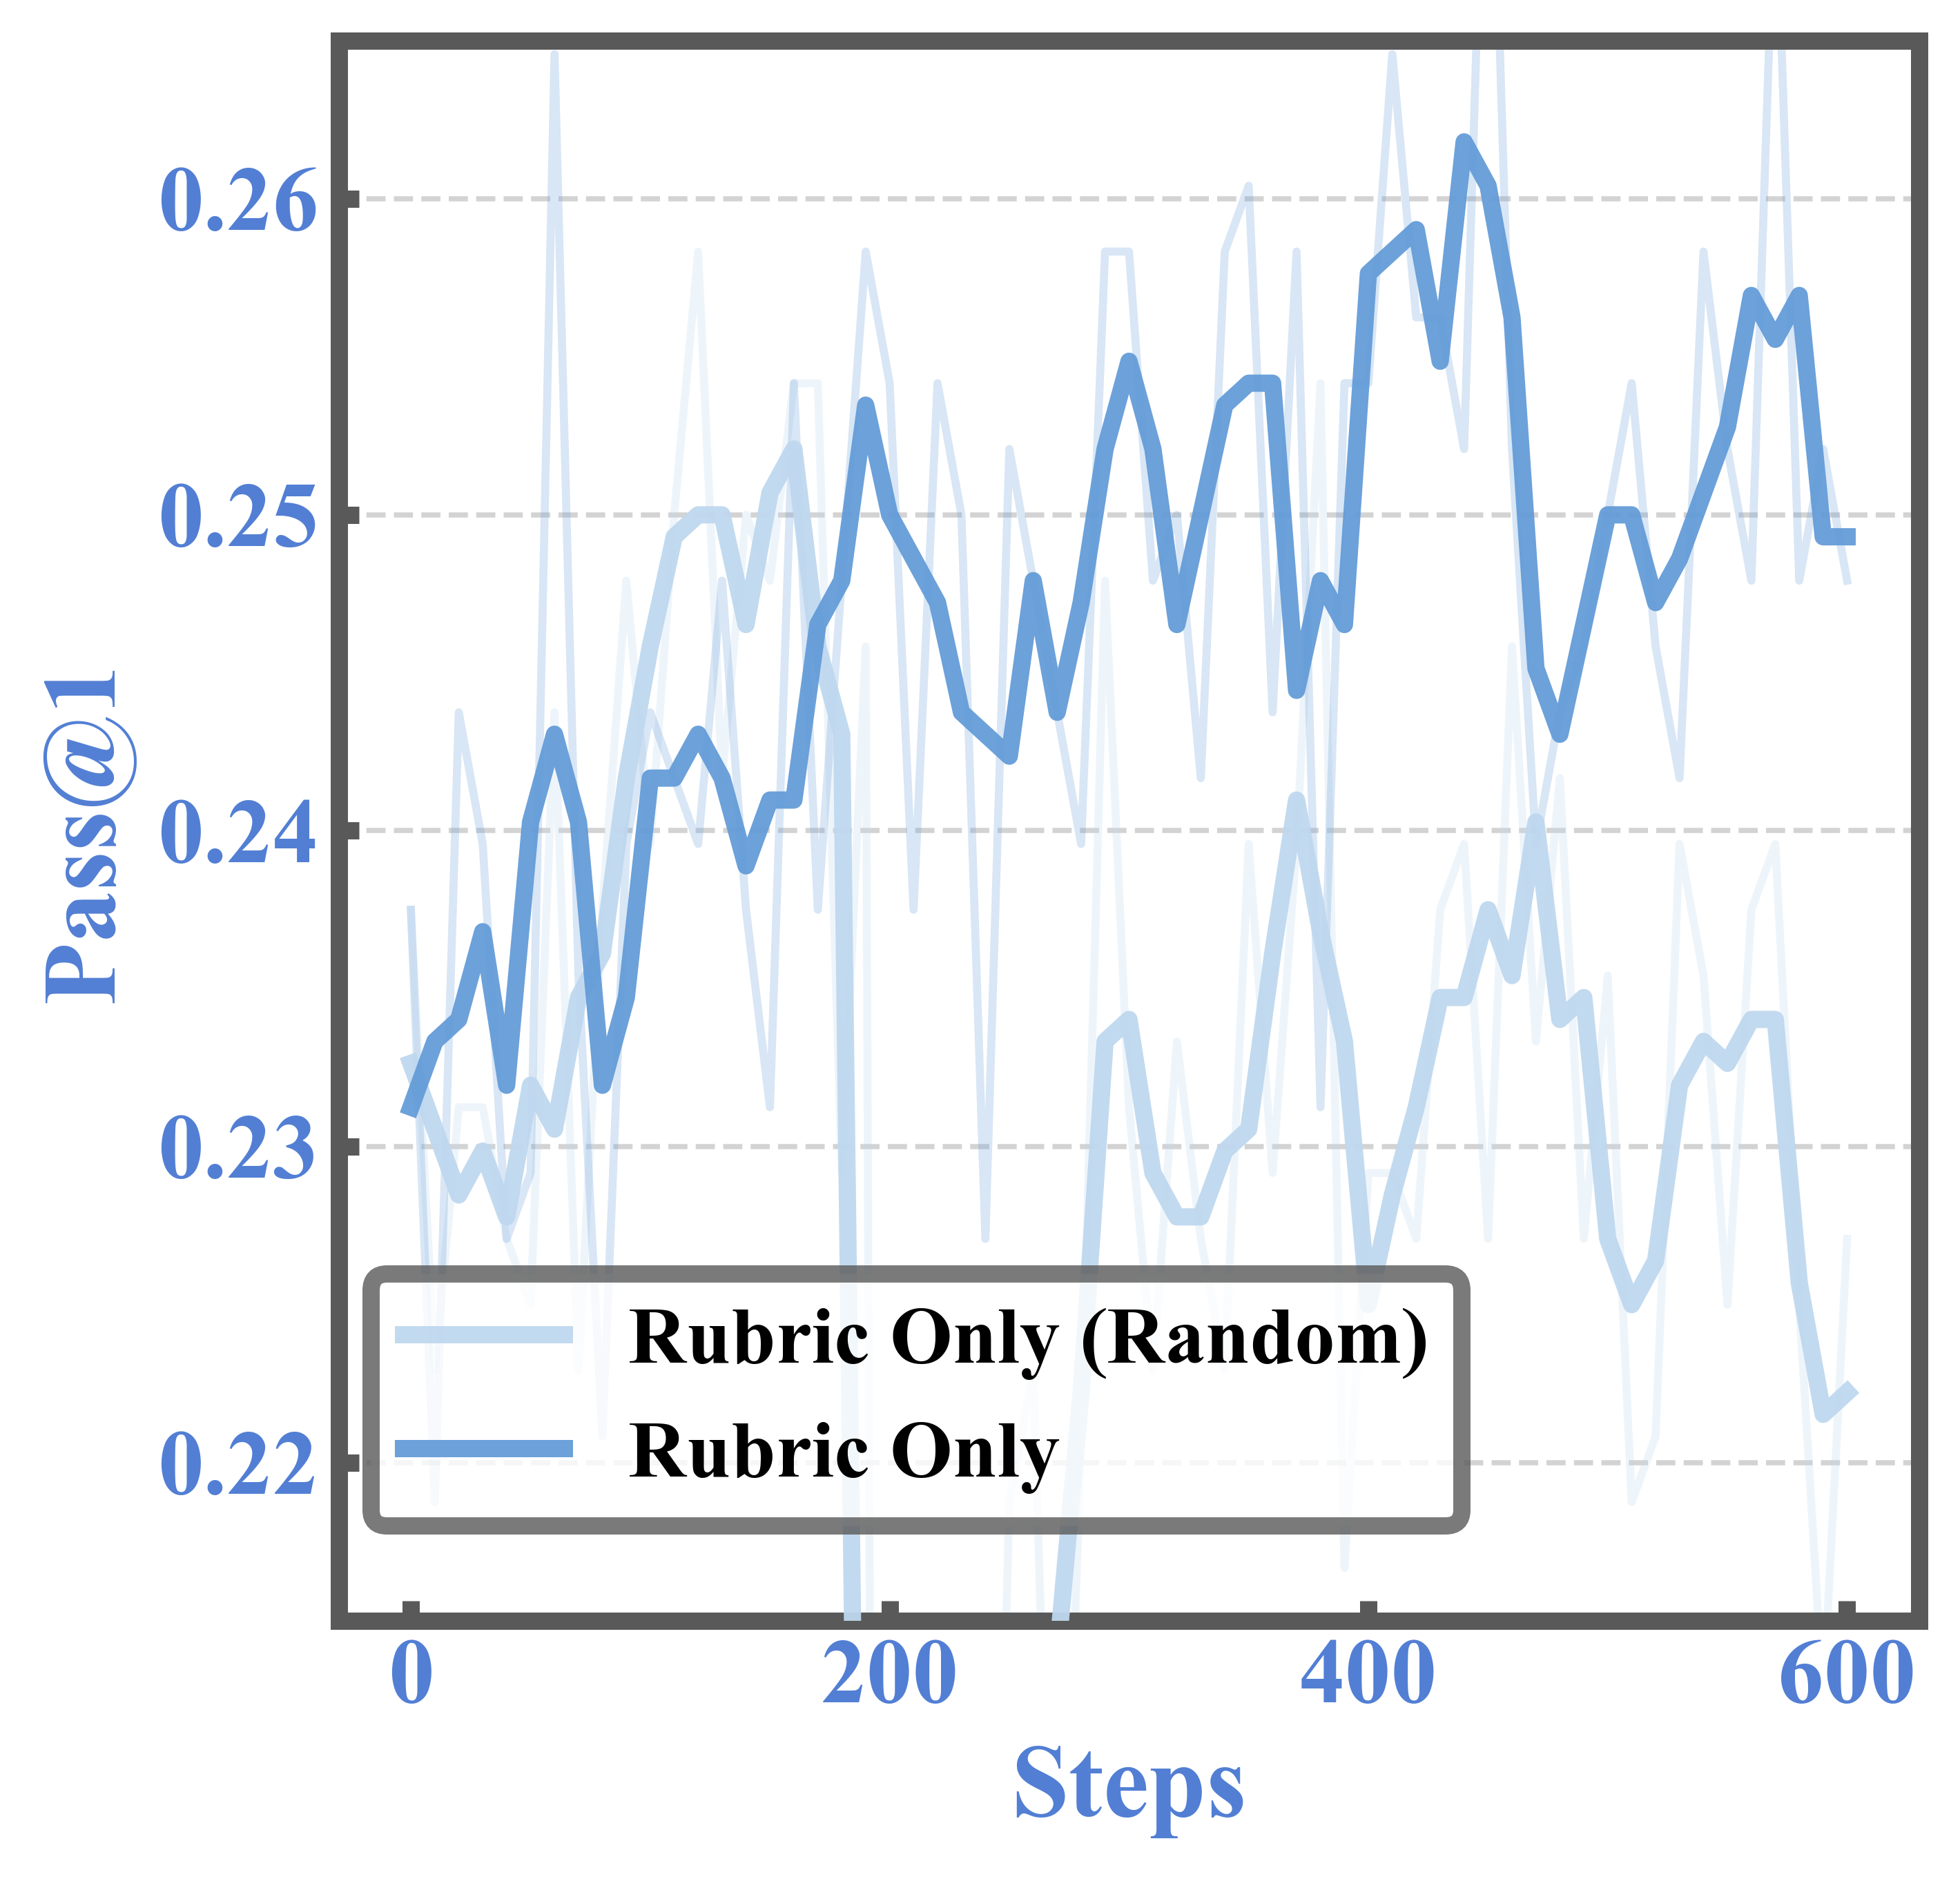
\includegraphics[width=\linewidth]{figures/exp/rubric_only/aime25_rubric_only.png}
    \caption{Accuracy on AIME25.}
    \label{fig:rubric-only-b}
  \end{subfigure}
  \vspace{-10pt}
  \caption{Accuracy dynamics when only rewarding CoTs. Even when rewarding CoTs with self-proposed rubrics without any outcome reward can bring consistent performance gain.}
  \label{fig:rubric-only}
  \vspace{-10pt}
\end{wrapfigure}

A key factor that determines the success of our method lies in whether the self-proposed and self-evolving rubrics can provide meaningful learning signals for RL. 
To verify this, we first conduct a preliminary experiment, considering an outcome-free setting that trains the model by \textbf{only rewarding CoTs based on self-proposed rubrics without any outcome rewards} (\ie $r^{\text{\textcolor{reasoner}{$Rea$}}} =  r_{cot}^{\text{\textcolor{reasoner}{$Rea$}}}$). 
If the model still learns to reason effectively under this setup, it would indicate that self-proposed rubrics can yield meaningful RL signals. 
We report the accuracy dynamics on reasoning tasks during the training in Figure \ref{fig:rubric-only}, where the bold lines are the rolling averaged performance with a window size of 3 and the slim and shallow lines are the original performance. 
We have the following observation:

\textbf{Self-proposed rubrics can provide meaningful CoT rewarding signals for RL training. }
As shown in this figure, by only rewarding CoTs with the self-proposed rubrics (\ie Rubric Only in the figure), the reasoning capability of the LLM shows consistent improvement during training. 
In contrast, when we assign random values between 0 and 1 as rubric rewards (\ie Rubric Only (Random) in the figure), the LLM fails to achieve performance improvements and even exhibits sudden performance drops during training around 200 steps. 
Such results show that the self-proposed and self-evolving rubrics can yield meaningful CoT rewarding signals, which lay an important foundation for our approach RLCER.

\subsection{(RQ2) Effectiveness of RLCER} \label{sec:main-performance}
Based on the reliability of self-proposed rubrics, we further test the effectiveness of combining both $r^{\text{\textcolor{reasoner}{$Rea$}}}_{outcome}$ and $r_{cot}^{\text{\textcolor{reasoner}{$Rea$}}}$ in RLCER. 
We compare RLCER with the vanilla RLVR which only considers the outcome reward, and report the performance comparison in Table \ref{tab:main-table}. 
Here, both RLCER and RLVR start from the SFT checkpoint.
We have the following observations: 


\textbf{RLCER outperforms the outcome-centric RLVR training. }
As shown in Table \ref{tab:main-table}, training with RLCER outperforms the vanilla RLVR across multiple datasets and multiple model sizes on average. 
Even when trained only on math datasets, RLCER also generalizes well on general reasoning tasks (\ie GPQA series.)
Additionally, we observe that the performance gain is more obvious on larger size models (\ie 8B models benefit more from RLCER than 4B models). 
Such phenomena validate the effectiveness of RLCER, which provides a ``free-lunch'' for improving the RL performance, by enhancing it with self-proposed and self-evolving rubrics. 
Case studies about the generated rubrics can be found in Appendix \ref{apdx:case-study}. 



\newcommand{\EMainTableScale}{0.99 }

\begin{table*}[!t]
\centering
\caption{The performance comparison across diverse reasoning benchmarks.}

\makebox[\linewidth][c]{%
  \resizebox{0.92\linewidth}{!}{%
    \begin{tabular}{cl|ccccccc}
    \toprule
    \multicolumn{2}{c|}{\textbf{}} &
    \multicolumn{7}{c}{\textbf{Datasets}} \\
    \textbf{Scale} & \textbf{Method} &
    \textbf{AIME2024} & \textbf{AIME2025} & \textbf{AMC2023} &
    \textbf{GPQA-Diamond} &
    \textbf{SuperGPQA-Eng} & \textbf{SuperGPQA-Med} & \textbf{SuperGPQA-Sci} \\
    \midrule

    % ===================== Scale: 4B =====================
    \multirow{4}{*}{4B}
    & Base
    & 11.25 & 6.46 & 31.09 & 7.77 & 18.50 & 14.25 & 15.44 \\
    & SFT
    & 17.29 & 18.96 & 59.53 & 24.43 & 31.69 & 28.25 & 27.81 \\
    \cmidrule(lr){2-9}
    & + RLVR
    & 29.38 & 30.21 & 79.53 & 44.16 & 39.75 & 28.50 & \textbf{42.88} \\
    & \cellcolor{lightgray}+ RLCER
    & \cellcolor{lightgray}\textbf{29.38}
    & \cellcolor{lightgray}\textbf{30.63}
    & \cellcolor{lightgray}\textbf{81.88}
    & \cellcolor{lightgray}\textbf{44.91}
    & \cellcolor{lightgray}\textbf{40.19}
    & \cellcolor{lightgray}\textbf{31.63}
    & \cellcolor{lightgray}41.81 \\
    \midrule\midrule

    % ===================== Scale: 8B =====================
    \multirow{4}{*}{8B}
    & Base
    & 11.46 & 9.58 & 42.34 & 24.37 & 33.06 & 24.69 & 23.63 \\
    & SFT
    & 22.29 & 23.75 & 66.41 & 31.72 & 36.00 & 33.75 & 35.19 \\
    \cmidrule(lr){2-9}
    & + RLVR
    & 34.79 & 32.50 & 84.53 & 46.56 & 42.94 & \textbf{38.31} & 48.81 \\
    & \cellcolor{lightgray}+ RLCER
    & \cellcolor{lightgray}\textbf{37.50}
    & \cellcolor{lightgray}\textbf{33.33}
    & \cellcolor{lightgray}\textbf{86.41}
    & \cellcolor{lightgray}\textbf{48.77}
    & \cellcolor{lightgray}\textbf{45.00}
    & \cellcolor{lightgray}36.50
    & \cellcolor{lightgray}\textbf{50.25} \\

    \bottomrule
    \end{tabular}
  }%
}

\label{tab:main-table}
\end{table*}

\subsection{(RQ3) Mechanism of Rubrics Self-Evolving} \label{sec:rubrics-self-evolving}


In this section, we study how the rubrics self-evolving affects training within the RLCER framework (\ie the role of the reward $r_{evolving}^{\text{\textcolor{rubricator}{$Rub$}}}$). 
To study this, we conduct an ablation study on the 8B-sized model by abandoning the evolving reward $r_{evolving}^{\text{\textcolor{rubricator}{$Rub$}}}$, and the rubricator is only rewarded with the format reward. 
We report the training dynamics in Figure \ref{fig:ablation-perf} and Figure \ref{fig:ablation-study-wrap} including the averaged performance (\ie averaged accuracy among AIME2024, AIME2025, and AMC2023), the averaged correlation between rubrics satisfaction and final answer correctness (\ie $\mathtt{corr}(\mathbf v_k,\mathbf z)$), and the CoT reward of the reasoner (\ie $r_{cot}^{\text{\textcolor{reasoner}{$Rea$}}}$). 
The performance is reported as the rolling average of 5 scores for a clearer demonstration, where the bold lines report the rolling average scores and the shallow and slim lines report the raw scores.
We have the following observations:


\begin{wrapfigure}{r}{0.52\textwidth}
  \vspace{-10pt}
  \centering

  \begin{subfigure}[t]{0.48\linewidth}
    \centering
    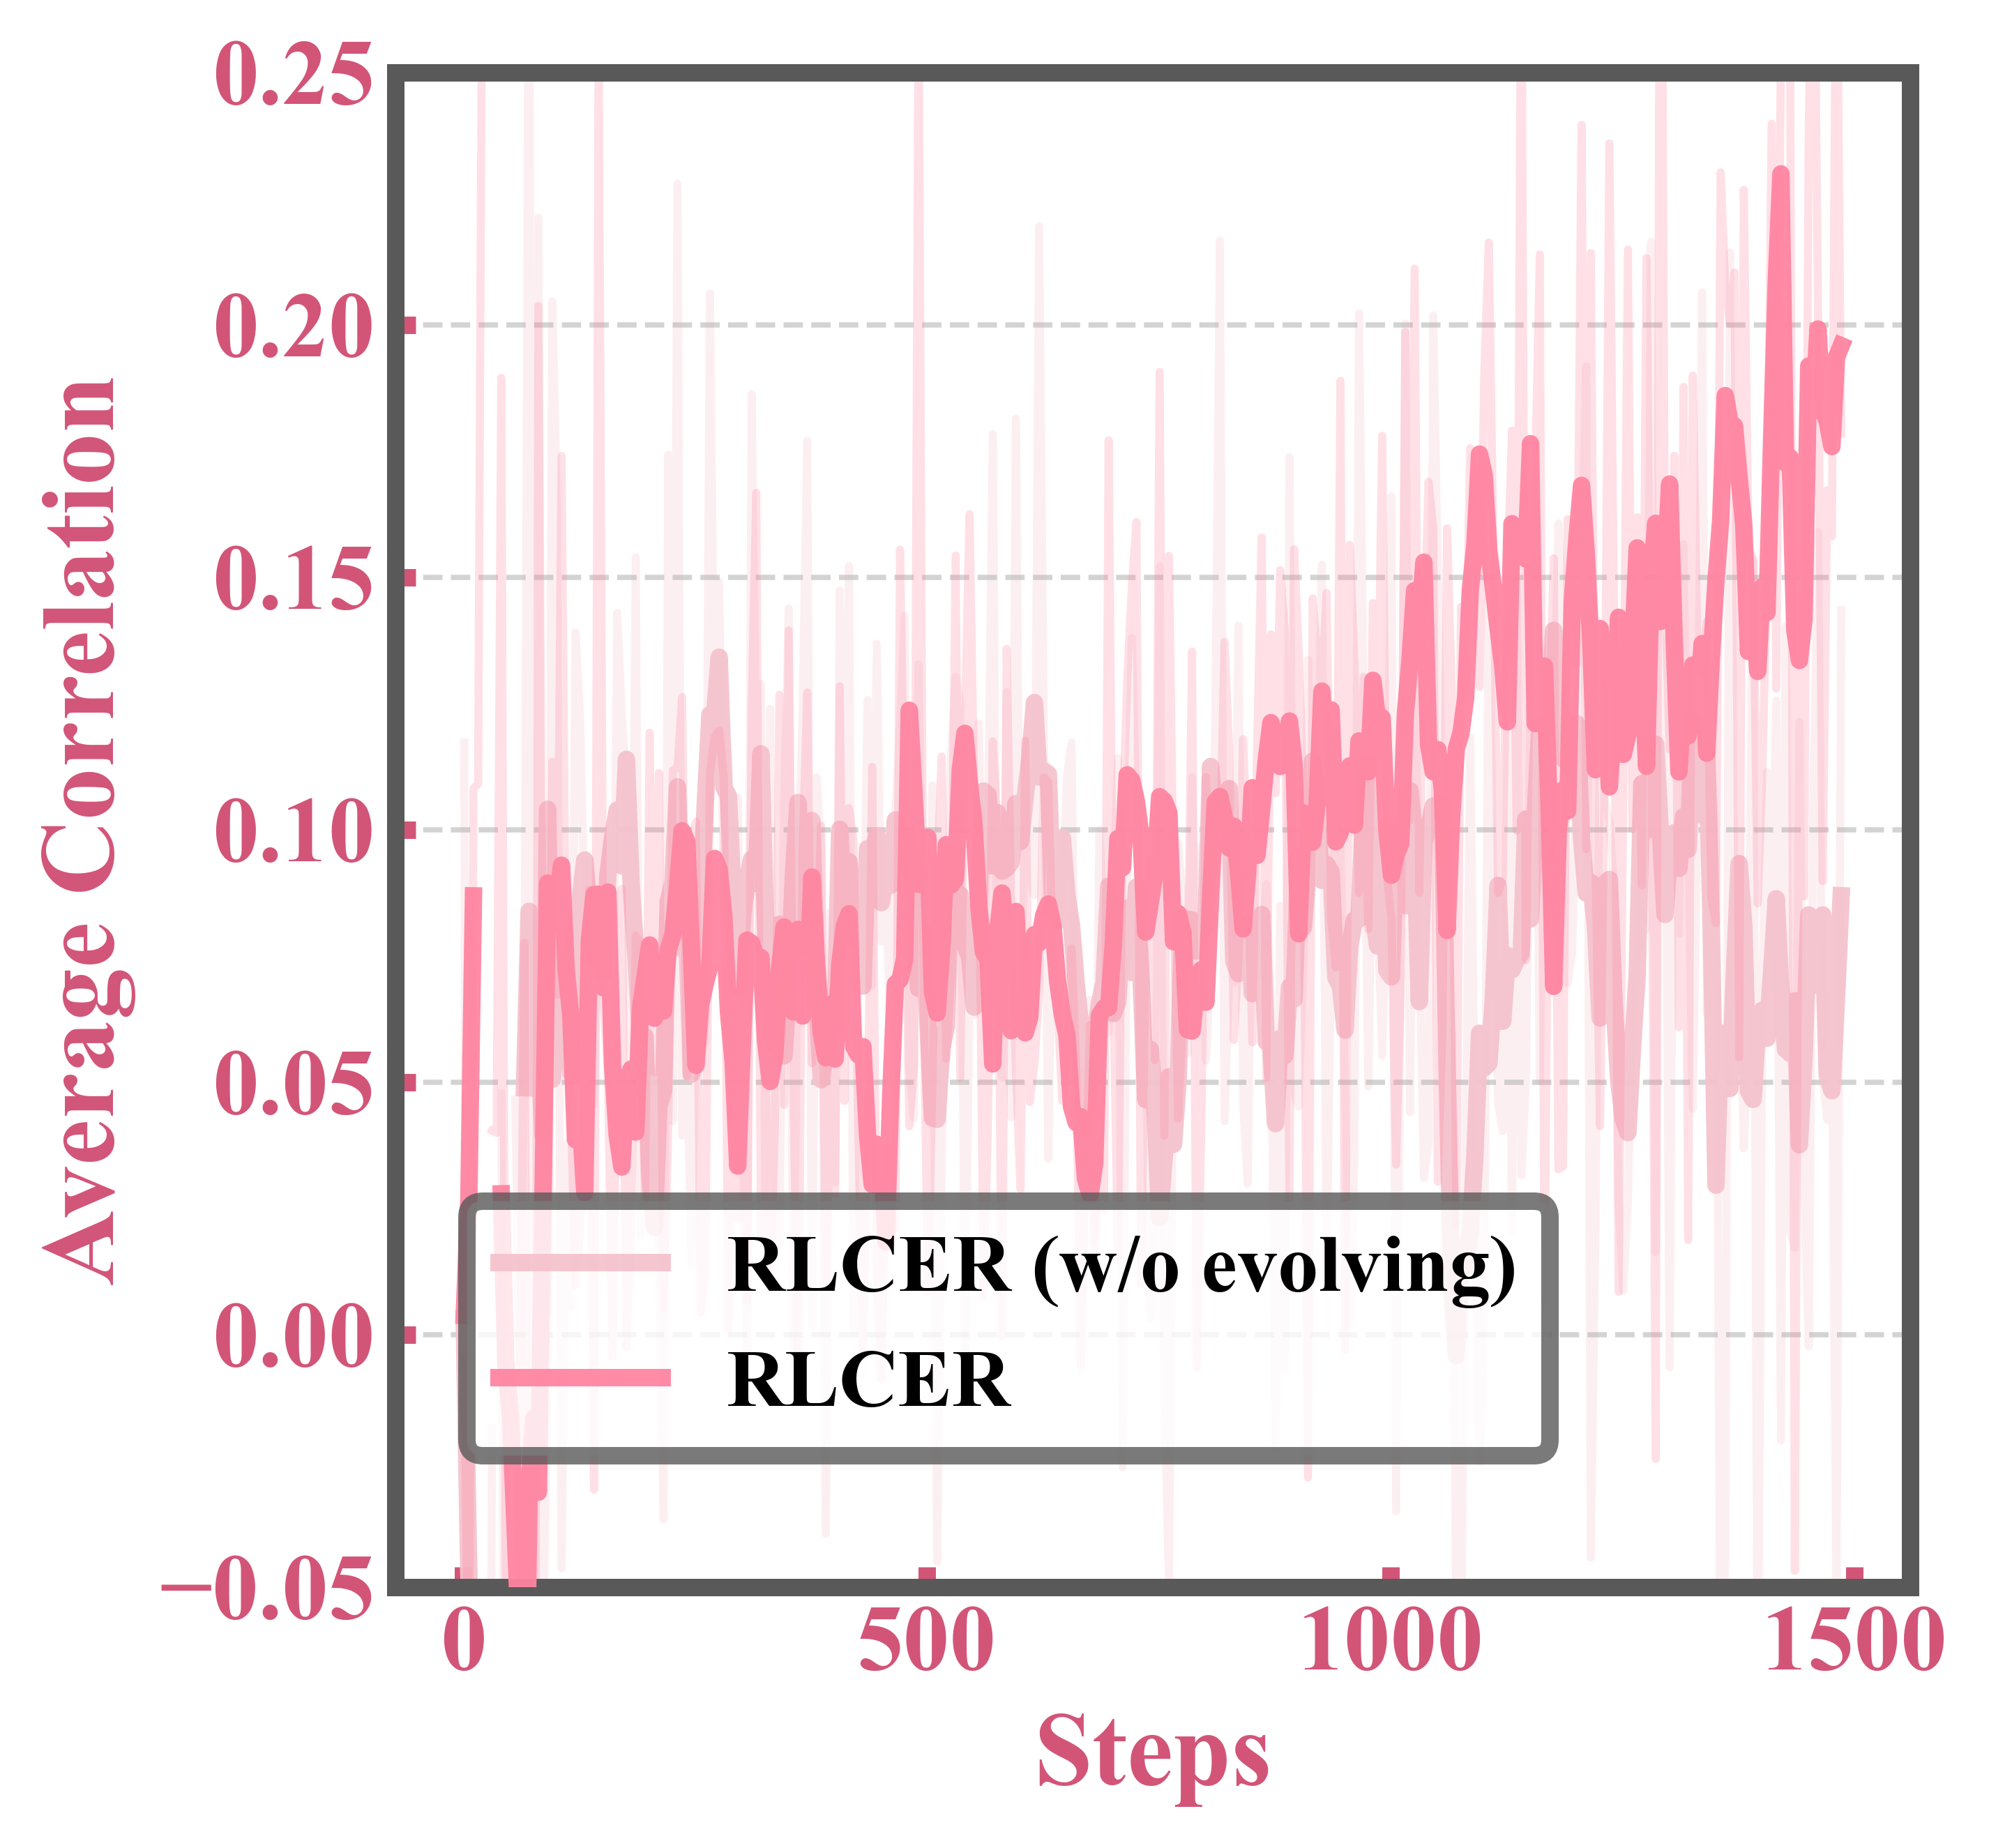
\includegraphics[width=\linewidth]{figures/exp/evolving_ablation/abl_corr.png}
    \subcaption{Correlation dynamics.}
    \label{fig:ablation-a}
  \end{subfigure}\hfill
  \begin{subfigure}[t]{0.463\linewidth}
    \centering
    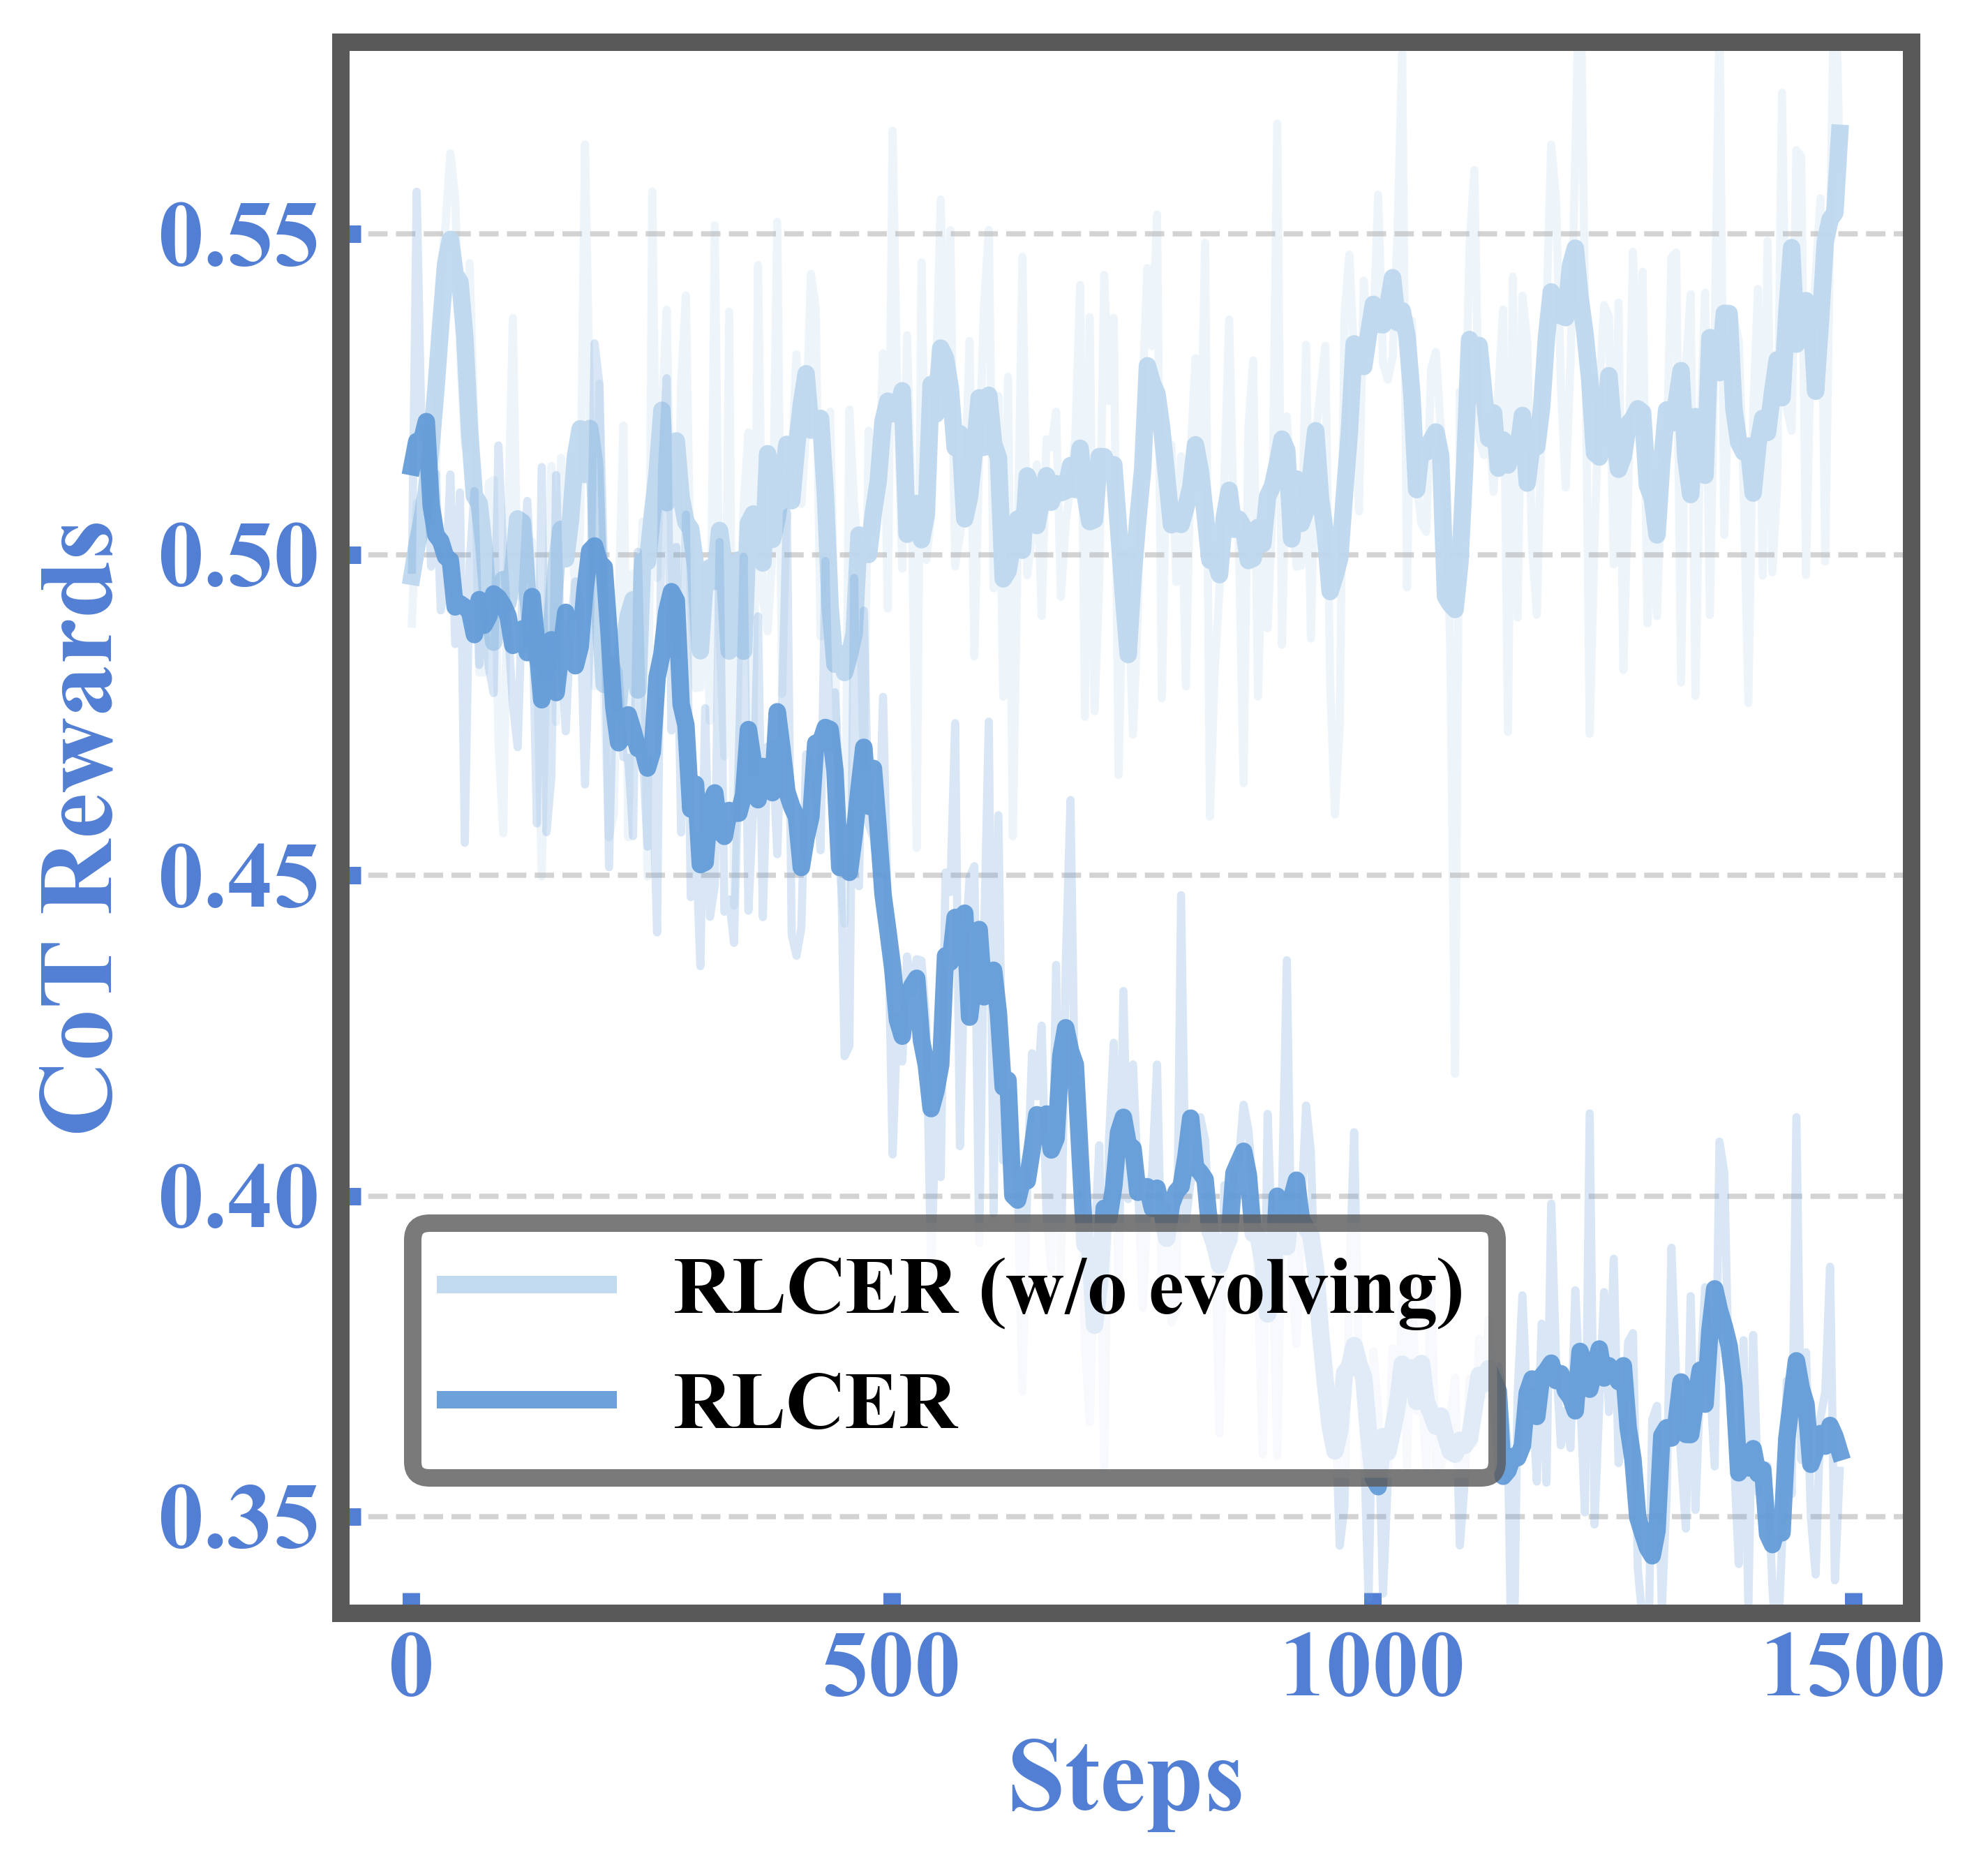
\includegraphics[width=\linewidth]{figures/exp/evolving_ablation/abl_cot_rewards.png}
    \subcaption{$r_{cot}^{\text{\textcolor{reasoner}{$Rea$}}}$ dynamics.}
    \label{fig:ablation-b}
  \end{subfigure}

  \vspace{-8pt}
  \caption{The effect of self-evolving on correlation and CoT-reward dynamics.}
  \label{fig:ablation-study-wrap}
  \vspace{-16pt}
\end{wrapfigure}

\textbf{Self-evolving rubrics enable better performance. }
As shown in Figure \ref{fig:ablation-perf}, by rewarding with $r_{evolving}^{\text{\textcolor{rubricator}{$Rub$}}}$, RLCER exhibits a more stable learning curve and gradually outperforms the ablation version (\ie RLCER (w/o evolving)). 
Additionally, both RLCER and RLCER (w/o evolving) outperform the naive RLVR method as it quickly converges to a sub-optimal performance.
Such phenomena show the effectiveness of self-evolving in enhancing reasoning. 

\textbf{Self-evolving with $r_{evolving}^{\text{\textcolor{rubricator}{$Rub$}}}$ enables more informative rubrics. }
We further analyze whether self-evolving enables the policy model to propose better rubrics.
As shown in Figure \ref{fig:ablation-a}, the averaged correlation between rubric satisfaction and final answer correctness (\ie $\mathtt{corr}(\mathbf v_k,\mathbf z)$) increases along the training process, while the ablation baseline shows an unchanged correlation. 
This indicates that self-evolving enables the policy model to gradually propose more informative rubrics that better align with the final answer correctness. 
Additionally, with such evolved rubrics, it gradually becomes harder to gain the CoT reward $r_{evolving}^{\text{\textcolor{rubricator}{$Rub$}}}$ as the Figure \ref{fig:ablation-b} shows a decreasing trend during the RLCER training. 
While the ablation baseline’s rubrics can be gradually satisfied by $\pi_{\theta}^{\text{\textcolor{reasoner}{$Rea$}}}$ as $r_{evolving}^{\text{\textcolor{rubricator}{$Rub$}}}$ increases. Such results highlight the importance of rubrics self-evolving.

\subsection{(RQ4) Effectiveness of Rubrics as In-prompt Reasoning Hints} \label{sec:rubrics-as-hint}

\begin{wrapfigure}{r}{0.52\textwidth}
  \vspace{-10pt}
  \centering
  % Crop top/bottom to make the square placeholder look wide
  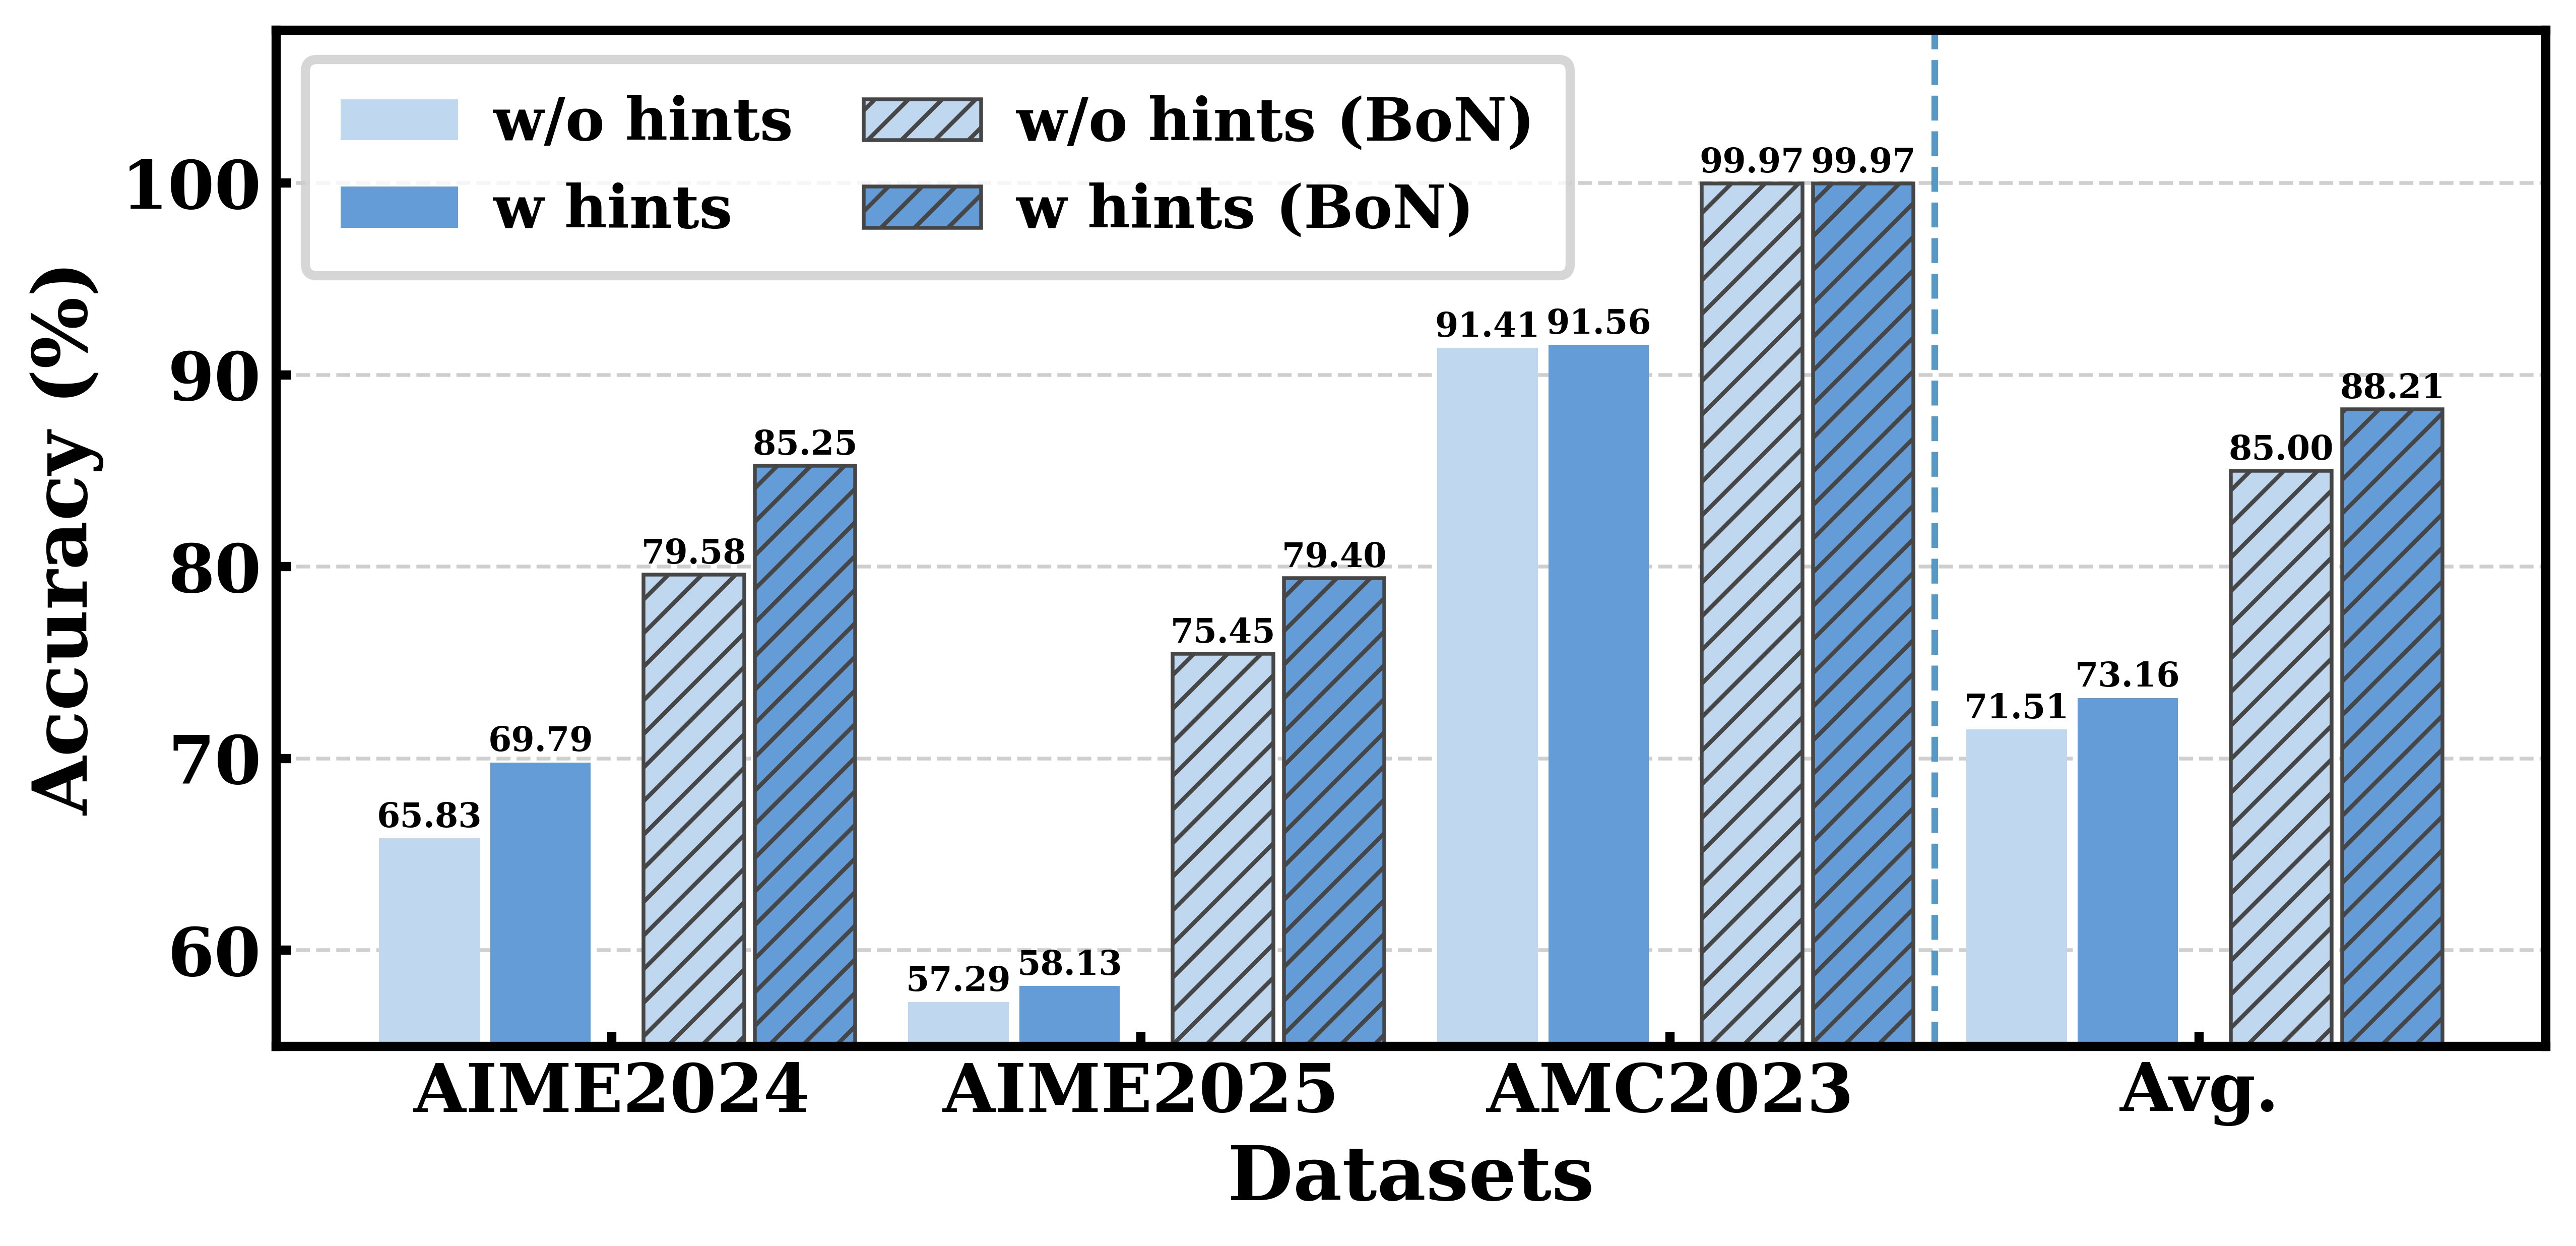
\includegraphics[width=\linewidth]{figures/hints/hints.png}
  \vspace{-20pt}
  \caption{Performance with rubrics as in-prompt hints.}
  \label{fig:rubrics-as-hint}
  \vspace{-10pt}
\end{wrapfigure}

In this section, we attempt to understand how the generated rubrics can guide the model toward better reasoning. 
While we have verified that self-proposed and self-evolved rubrics can generate valid signals for rewarding CoTs, the mechanism through which these rubrics implicitly steer reasoning processes remains elusive, largely because the underlying reward signals are difficult to analyze.
To this end, we explicitly employ these self-proposed rubrics as in-prompt hints, and evaluate the model’s reasoning performance under this setup. 
If incorporating the rubrics into the prompt yields performance improvements, it demonstrates that the rubrics offer valid guidance for the reasoning path. 
We report the performance of Qwen3-8B with a max response length of 20480 in Figure \ref{fig:rubrics-as-hint}. 
As shown in the figure, when using generated rubrics as in-prompt hints, the performance improves, indicating that these rubrics can indeed guide better reasoning. 
Additionally, the performance of BoN (N=16) improved even further on the AIME datasets, indicating that the rubrics introduced as hints may incentivize LLMs to conduct more exploration. 


\renewcommand{\arraystretch}{0.9}
